\title{\bf Telescopes}

\section{Basics \& Nomenclature}

Telescopes are the fundamental tool of astronomers, with a handful of
exceptions ($\gamma$-ray detectors, cosmic ray detectors, neutrino
detectors, and gravitational wave detectors). 

Telescope optics are design to do two things: to collect a lot of
light; arrange the collection process to separate the light according
to its incoming direction. Detectability of objects depends on how
many photons, or equivalently how much energy, is collected. This
number is the product of $f_\nu A t \Delta\nu$, where $A$ is the
telescope area, $t$ is the length of exposure, and $\Delta\nu$ is the
width of detector bandpass.

The two basic types of telescope are {\it refracting} and {\it
reflecting} telescopes. Refractors transmit the light through
transparent media with refractive indices different than air, bending
it through Snell's Law. Reflectors are mirrored surfaces, in the
optical typically aluminized, whose shapes manipulate beams of light
in the desired fashion. Reflecting telescopes virtually always have
some refracting elements inside of them.

For astronomical telescopes, they always focus at infinity, meaning
they are designed such that parallel rays of light are focused to a
single point in the focus of the telescope.  Typically, there is some
axis of symmetry to the telescope and rays parallel to this axis are
{\it on-axis}, and it is typically here that the telescope is designed
to have best focus. {\it Off-axis} rays may be well focused as well,
but as the angle off-axis becomes larger the rays do not all
converge. Off-axis rays can be obstructed by either parts of the
optics or part of the telescope structure, and generally are more
obstructed than on-axis rays; this effect is known as {\it
vignetting}.  The usable {\it field of view} of the telescope is
typically determined by the off-axis angle at which the beam is too
vignetted or too badly focused to be usable for the desired purpose.

% Below is a picture of a lens diagram for a refracting telescope. The
% lens has a focal length, which is what determines how far beyond the
% lens a set of parallel, on-axis rays will come to focus. Physically,
% the lens is bending the light according to Snell's law, and the shape
% of the front and back surface of the lens as a function of its radius
% is what conspires to direct all the on-axis light to the focus.

A key parameter in the optical design is the {\it focal ratio}, or
{\it $f$-ratio}, the ratio of the focal distance $f$ to the aperture
diameter $D$. This is usually expressed in the form ``$f/N$'' (which
is not a division), where $N = f/D$. This ratio determines the angular
size of the beam that converges on the focal point; in more complex
optical configurations, it is this beam width that defines the
$f$-ratio. The smaller the $f$-ratio the more the light is being bent;
this means that off-axis rays will usually fall out of focus more
quickly with off-axis angle without very careful design.

Slightly off-axis light focuses to a slightly offset spot in the focal
plane. The relationship between the off-axis angle and physical radius
in the focal plane from the on-axis focus (sometimes known as the {\it
plate scale}) is determined by the $f$-ratio. Specifically:
\begin{equation}
{\rm d}x \approx f {\rm d}\theta
\end{equation}
so:
\begin{equation}
\frac{{\rm d}x}{{\rm d}\theta} \approx f
= \left(\frac{f}{D}\right) D
\left(\frac{10^6~\mu{\rm m}}{{\rm m}}\right)v
\left(\frac{\rm rad}{(180/\pi)(3600)~{\rm arcsec}}\right)
= \left(\frac{f}{D}\right) \frac{D}{{\rm m}}
\left(4.85 \frac{\mu{\rm m}}{\rm arcsec}\right)
\end{equation}
or inversely as 
\begin{equation}
\label{eq:platescale}
\frac{{\rm d}\theta}{{\rm d}x} \approx 
\left(\frac{f}{D}\right)^{-1} \frac{{\rm m}}{D}
\left(0.206\frac{\rm arcsec}{\mu{\rm m}}\right)
\end{equation}
This equation holds given the final $f$-ratio of any of the optical
systems we describe here. It means the smaller the $f$-ratio, or the
smaller the telescope size, the more angular coverage per unit area
there is.

There are three major limitations of refracting telescopes:
\begin{ditemize}
\item The index of refraction of light in lens materials varies with
wavelength. This means that the focal length depends on wavelength as
well, and only one wavelength can be in perfect focus. This effect is
known as {\it chromatic aberration} and is a limitation of refracting
telescopes (and affects reflecting telescopes with refracting optics
inside them). It is somewhat mitigated with large $f$-ratios, which
minimize the angular deflections.
\item Mitigating chromatic aberration and maintaining focus off-axis
both drive the telescope design to reasonably high $f$-ratios. With a
refractor, this inevitably lengthens the telescope structure in ways
that can be avoided with reflecting telescope. A very long telescope
necessitates a large dome, a more difficult engineering problem to
manipulate the telescope, and more difficulty in minimizing flexure
(bending) in the system.
\item
The practical size limit for refracting optical elements in the
optical is about 1 meter. It is extremely hard to create precise
optical elements larger than that size at finite cost.
\end{ditemize}
These considerations drove astronomers in the late 1800s and early
1900s to move to reflecting telescopes for large telescope
applications.

The principles of reflecting telescopes to first order can be
understood through the mathematics of conic sections: parabolae,
ellipses, and hyperbolae. Reflecting surfaces in telescopes are close
approximations to axisymmetric surfaces of revolution whose radial
shape is defined by these conic sections. Conic section can be defined
in terms of their two {\it foci}. One of their mathematical properties
is that at any point on the curve, the normal to the curve bisects the
directions to the foci. This mathematical property has the consequence
that a ray of light emitted from the direction of one focus will be
reflected from the surface along the direction defined by the other
focus.

Astronomical observations are almost invariably of extremely distant
objects, the light rays from which are parallel to each other. This
corresponds to a {\it focus at infinity}. A conic section with one
focus at infinity and one at finite distance is a parabola. Therefore,
if a parabolic mirror is aligned with these rays, they will be
reflected towards the other focus of the parabola. A simple design for
a telescope therefore is to put a detector at the focus of a parabolic
mirror, referred to as the {\it primary}. A slight variant known as
the Newtonian design is to direct this {\it prime focus} with a flat
pickoff mirror.

More complex designs are possible with multiple curved surfaces. The
general principle behind these designs are to use the fact that conic
sections like ellipsoids and hyperboloids have two foci. A {\it
secondary mirror} is designed to have one focus coincide with the
prime focus; the reflective surface then will refocus the light to its
other focus. A third ({\it tertiary}) mirror is used in some designs
(for example in the Large Synoptic Survey Telescope).

There are multiple purposes of the extra surfaces. They allow the
focus to be redirected to a mechanically more convenient spot than the
primary. They allow freedom to manipulate the $f$-ratio of the
beam. For wide-angle observations, the design of the primary,
secondary, and other mirror shapes can be slightly perturbed from the
conic section ideals to allow off-axis light to remain in better focus
(at the cost of focus on-axis). In operation, that they are smaller
than the primary makes them more easily adjustable in real time to
perform focus changes and tip/tilt corrections for image motion.

Many reflecting telescope systems have {\it correctors}, which are
refractive elements near their focus used to reduce distortions across
the field of view.

The diffraction-limited point spread function of a telescope is
related to its aperture. The ``pupil'' of the system is the image of
the aperture including any obstructions in the optical path, for a
plane wave arriving at the telescope aperture. In detail, optical
imperfections will also lead to phase differences as a function of
position in the pupil. Thus the ``complex pupil function'' $A
e^{i\phi}$ gives the throughput $A$ and phase shift $\phi$ of each
point in the aperture. A consequence of Huygen's Principle of
diffraction isthat the plane wave is focused onto a spot with an
intensity function with a spatial form that is the square of the
Fourier transform of the complex pupil function.

For the simplest aperture, a circular one with no phase shifts, the
width of the diffraction-limited point spread function is related to
the aperture diameter $D$. Specifically:
\begin{equation}
\label{eq:psf_tophat}
I(x) \propto \left(\frac{J_1(x)}{x}\right)^2,
\end{equation}
where $J_1$ is the first-order Bessel function and $x=\pi D \theta
/\lambda$. Here $\theta$ is the equivalent angle from the center of
the spot. 

Most of these general considerations hold for telescopes outside the
optical. However, the designs of these telescopes differ in
detail. From the UV through the mid-infrared they are usually quite
similar to the optical. High energy photons do not reflect easily off
aluminized surfaces, or near the normal to the surface. X-ray
observations therefore use gold-coated surfaces under ``grazing
incidence,'' with nested annular hyperboloid surfaces. Radio
telescopes simply require conductive surfaces and much lower
tolerances due to their longer wavelength, meaning they can be built
at fixed construction cost to much larger aperture than optical
telescopes. To avoid interference, radio telescopes also typically use
asymmetric sections of a paraboloid.

\section{Commentary}

Astrophysics and astronomy courses typically focus on the optical
aspects of telescopes and the nature of their detectors.  The
engineering aspects of telescopes, both in hardware and in software,
are not well covered in the astrophysics or in the engineering
disciplines.

\section{Key References}

\begin{itemize}
  \item
    {\it Design and Construction of Large Telescopes},
      \citet{bely03a}
\end{itemize}

\section{Order-of-magnitude Exercises}

\begin{enumerate} 
\item By considering two on-axis light rays each hitting each
    side of a telescope of diameter $D$ and interfering near the focal
    plane, estimate the diffraction limit in terms of the wavelength
    of light $\lambda$ and diameter $D$.

\begin{answer}
By Huygens' Principle, the two rays can be treated as each producing a
spherically outgoing wave from their location on the aperture. If the
two rays are in phase when they hit the perfectly constructed mirror,
they will constructively interfere exactly at focus. Near but slightly
off focus in the focal plane, they will not exactly interfere because
the distances from the mirror for each ray will be slightly different,
so their phases at this location will not be the same.  The size of
the central image can be characterized by the position of the first
null --- i.e. when the phase difference of the two rays becomes $\pi$,
so that they destructively interfere.

The path length from either aperture location to perfect focus is:
\begin{equation}
d = \sqrt{f^2 + \left(\frac{D}{2}\right)^2}, 
\end{equation}
where $f$ is the focal length.  For some $\delta$ in distance away
from perfect focus, the path length for one ray will be:
\begin{eqnarray}
d_L &\approx& \sqrt{f^2 + \left(\frac{D}{2} + \delta\right)^2} \cr
&\approx& \sqrt{d^2 + D\delta} \cr
&\approx& d \left(1 + \frac{D \delta}{2 d}\right),
\end{eqnarray}
and the other ray will have a slightly shorter path by the same
amount: 
\begin{eqnarray}
d_R &\approx& 
d \left(1 - \frac{D \delta}{2 d}\right).
\end{eqnarray}
The difference in angle that $\delta$ corresponds to relative to
incoming rays on the sky will be $\alpha \approx \delta / d$. That is,
the difference in focal plane distance $\delta$ corresponds to a
difference in $\alpha$ on sky for perfect geometric options. So we can
write the difference in path length in units relative to sky:
\begin{equation}
\Delta d = d_L - d_R = D \alpha.
\end{equation}

These two waves will destructively interfere when  $\Delta d = \lambda
/ 2$. This will be when:
\begin{equation}
\alpha = \frac{\lambda}{2 D}
\end{equation}
This of course is smaller than the first null for an Airy function,
because the Airy function involves the interference of {\it all} of
the waves coming from the surface of the mirror, many of which have
much smaller separations. But this argument shows how $\lambda/D$
enters the problem.
\end{answer}

\item The LSST telescope in Cerro Pachon has a diameter of $\sim 8$ m
    and is $f/1.4$ at its focus. To sample with at least two pixels
    per full-width half maximum (e.g. the Nyquist critical sampling)
    for the best atmospheric seeing in Chile it might encounter (about
    0.5 arcsec FWHM), what must the detector pixel size be?

\begin{answer}
To sample with two pixels per FWHM requires $\theta\sim 0.25$ arcsec
$\sim 1.212 \times 10^{-6}$ radians.  The focal distance is $N D =
1.4\times 8 {\rm ~m} = 11.2 {\rm ~m}$, and we find therefore that the
pixel size should be $\theta N D \sim 13~\mu$m (or equivalently
consult Equation \ref{eq:platescale}). The actual LSST design has 10
$\mu$m pixels.
\end{answer}

\item Assuming that telescope diffraction is the dominant effect
defining the PSF of a telescope, how accurate does its mirror have to
    be in order to limit the change in the central flux of the PSF due
    to imperfections to less than 10\%? In the $X$-rays? the optical?
    the radio?

\begin{answer}[Author: Nanoom Lee]
Let's approximate the telescope as consisting of just two patches of
mirror and consider the interference from those two patches. If they
are perfectly accurately placed than the intensity of light at the
center of focus is just proportional to the the time-averaged square
of the electric field due to each one added together:
\begin{eqnarray}
I &\propto& \left\langle
\left|
\sin\left(\omega t - \frac{2\pi d}{\lambda}\right) +
\sin\left(\omega t - \frac{2\pi d}{\lambda}\right)
\right|^2 \right\rangle \cr
&\propto& 4 \left\langle
\left|
\sin\left(\omega t - \frac{2\pi d}{\lambda}\right)^2
\right|^2 \right\rangle
\end{eqnarray}
where $\lambda$ is the wavelength of the light, $\omega$ is its
frequency, and $d$ is the path length from the given mirror.

Now let's assume the mirror are not perfectly placed. This corresponds
to the case that a full mirror is not perfectly figured and
polished. The waves will no longer perfectly constructively interfere.
We quantify the level of imperfection as a small difference in the
path length, $\Delta d = \delta$. Then, the light ray reflected at
this point will interfere with the other light ray and change the
intensity of the light at the focus.
\begin{eqnarray}
I' &\propto& \left\langle\left|
\sin\left(\omega t - \frac{2\pi d}{\lambda}\right) +
\sin\left(\omega t - \frac{2\pi
(d+\delta)}{\lambda}\right)\right|^2\right\rangle \cr
&\propto& \left\langle\left[
\sin\left(\omega t - \frac{2\pi d}{\lambda}\right)^2 +
\sin\left(\omega t - \frac{2\pi (d+\delta)}{\lambda}\right)^2
+ 2 \sin\left(\omega t - \frac{2\pi d}{\lambda}\right)
\sin\left(\omega t - \frac{2\pi (d+\delta)}{\lambda}\right)
\right]\right\rangle \cr
&\propto& \frac{I}{2}
+ \left\langle 2 \sin\left(\omega t - \frac{2\pi d}{\lambda}\right)
\sin\left(\omega t - \frac{2\pi (d+\delta)}{\lambda}\right)
\right\rangle
\end{eqnarray}
where in the last line we just use the fact that the time average of
$\sin^2(\omega t + \phi)$ is independent of $\phi$. Considering the
second term, we can use trigonometric identities to simplify it:
\begin{eqnarray}
\left\langle 2 \sin\left(\omega t - \frac{2\pi d}{\lambda}\right)
\sin\left(\omega t - \frac{2\pi (d+\delta)}{\lambda}\right)
\right\rangle
&=& 
\left\langle 2 \sin^2\left(\omega t - \frac{2\pi d}{\lambda}\right)
\cos\left(\frac{2\pi \delta}{\lambda}\right)
\right\rangle + \cr
& &
\left\langle 2
\sin\left(\omega t - \frac{2\pi d}{\lambda}\right)
\cos\left(\omega t - \frac{2\pi d}{\lambda}\right)
\sin\left(\frac{2\pi \delta}{\lambda}\right)
\right\rangle \cr
&=& 
\left\langle 2 \sin^2\left(\omega t - \frac{2\pi d}{\lambda}\right)
\cos\left(\frac{2\pi \delta}{\lambda}\right)
\right\rangle
\end{eqnarray}
where in the last line we drop the time average sine times cosine,
which will be zero. Then we find:
\begin{eqnarray}
\frac{I'}{I} &=& \frac{1}{2} \left(1 + 
\cos\left(\frac{2\pi \delta}{\lambda}\right) \right) \cr
&\approx& 1 - \frac{1}{4}\left(\frac{2\pi\delta}{\lambda}\right)^2
\end{eqnarray}
The question asks when this ratio is 0.9, which will be when:
\begin{equation}
\frac{\delta}{\lambda} \approx \frac{1}{\sqrt{10} \pi} \approx \frac{1}{10}
\end{equation}
So about $\delta \sim 0.1$ \AA\ for X-rays, $\sim 0.05~\mu$m  in the
optical, and $\delta \sim 1~$mm for 
the cm-wavelength radio.
 \end{answer}
\end{enumerate} 

\section{Analytic Exercises}

\begin{enumerate}
\item The Cassegraine design and Gregorian design both involve a
curved secondary redirecting the focus along the original primary
focal axis. In the Cassegraine, the secondary is before the prime
focus. In the Gregorian it is after. What are the shapes of each of
these secondary choices: ellipsoid, paraboloid, or hyperboloid? Draw
the mirrors and the paths for on-axis light in the two cases.

\begin{answer}[Author: Kate Storey-Fisher]
The Cassegraine secondary mirror needs to intercept the light from the
primary mirror before it reaches the focus, and redirect it through a
hole in the primary. This is achieved a by a convex hyperbolic mirror.

\begin{figure}[!h]	
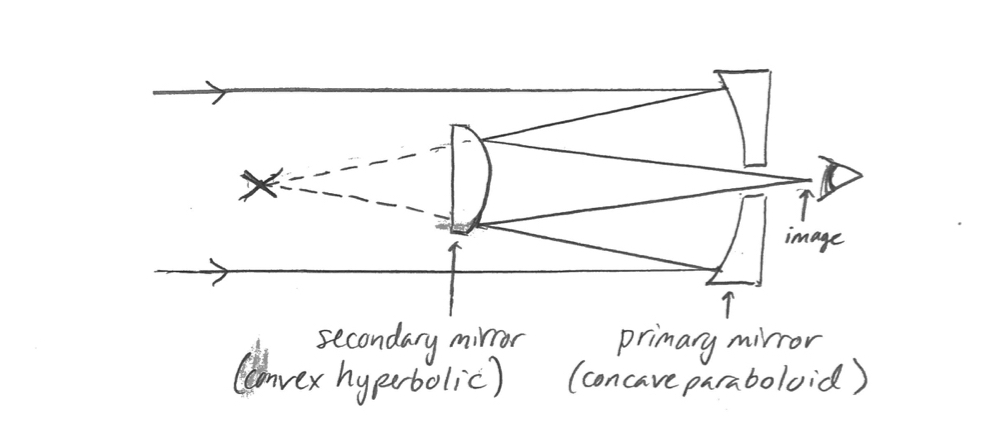
\includegraphics[width=1\columnwidth]{figures/cassegraine.jpg}
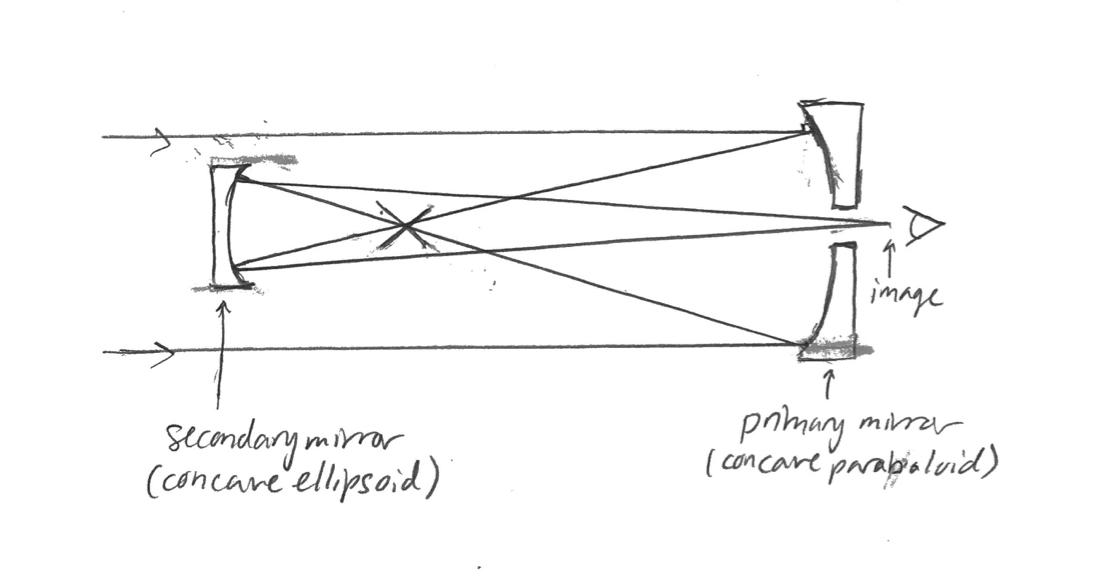
\includegraphics[width=1\columnwidth]{figures/gregorian.jpg}
\caption{The mirror design for the Cassegraine (top) and Gregorian
(bottom) telescopes.}
\label{fig:cassgreg}
\end{figure}

This type of reflector has two focii, one behind and one in front of
the mirror. It will reflect light directed at one focus to the
other. In the Cassegraine, the back focus is aligned to the focus of
the primary mirror so they share one focus. Then the front focus is
past the primary mirror, where the image will appear. This is shown in
the top panel of Figure~\ref{fig:cassgreg}.

The Gregorian design allows the light reflected from the primary
mirror to cross through the focus before hitting the secondary
mirror. This mirror is a concave ellipsoid, directing the light
through the hole in the primary to form an image. The closer focus of
the ellipsoid coincides with the primary mirror's focus. The shape
ensures there are no spherical aberrations. This design is shown in
the bottom panel of Figure~\ref{fig:cassgreg}.


\end{answer}

\item In the two above cases, there usually needs to be a hole in the
primary mirror (and the secondary would obstruct that area anyway).
What is the analytic form of the diffraction limited point spread
function for an aperture like this?
\end{enumerate}

\begin{answer}[Author: Nick Faucher]

The diffraction-limited point spread function of a telescope is equal
to the squared modulus of the Fourier transform of the pupil. In this
case, we are considering a pupil which allows light to pass through a
circular aperture of radius b, excluding the center of the circle out
to radius a with a $<$ b:
\begin{equation}
f(r,\theta)= 
\begin{cases}
   0,& \text{if } r < a\\
   1,& \text{if } a \leq r \leq b\\
    0,              & \text{otherwise}
\end{cases}
\end{equation}

The two-dimensional Fourier transform for a single circular aperture
with radius b can be written in polar coordinates as

\begin{equation}
\mathcal{F}(k,\phi)= \int_{0}^{b} \int_{0}^{2\pi} e^{i \: k \: r \: \cos(\theta-\phi)} d\theta \: r \: dr
\end{equation}

Since the Fourier transform of a circularly symmetric function is also circularly symmetric, we can let $\phi=0$ to simplify the integral:

%\begin{equation}
\begin{align*}
\mathcal{F}(k) &= \int_{0}^{b} \int_{0}^{2\pi} e^{i \: k \: r \: \cos(\theta)} d\theta \: r \: dr \\ \\
&= 2 \: \pi \int_{0}^{b} J_0 (k \: r) r \: dr
\end{align*}
%\end{equation}

Where $J_0$ is the $0^{th}$ order Bessel function. Through the change of variables $u=k \: r$, we can  write the integral as 
\begin{equation}
\mathcal{F}(k) = \frac{2\pi}{k^2} \int_{0}^{k \: b} J_0 (u) u \: du \\ \\
\end{equation}
which has the well known solution
\begin{equation}
\mathcal{F}(k) = \frac{2\pi}{k^2} J_1 (k \: b) k \: b  \\ \\
\end{equation}
or equivalently:
\begin{equation}
\mathcal{F}(k) = 2 \pi \: b^2 \bigg[ \frac{J_1 (k \: b)}{k \: b} \bigg]  \\ \\
\end{equation}
The wavenumber $k$ corresponds to a position in the focal plane
equivalent to some off-axis angle $\theta$; it turns out that (based
on the text below Equation \ref{eq:psf_tophat}) $k=2\pi\theta
/ \lambda$ (a future version of these solutions should explain why
those precise units!). Thus:
\begin{equation}
\mathcal{F}(\theta) = 2\pi \: b^2 \left[
\frac{J_1 (2\pi b \theta /\lambda)}{2\pi b \theta / \lambda} \right]  \\ \\
\end{equation}

To get the Fourier transform corresponding to Equation (1), we can
simply take the result from Equation (5) and subtract from it the same
equation with b replaced by a:
\begin{equation}
\mathcal{F}(\theta) = 2 \pi \: b^2 \bigg[
\frac{J_1 (2\pi b \theta/\lambda)}{2\pi b \theta / \lambda} \bigg] -
2 \: \pi \: a^2 \bigg[ \frac{J_1 (2 \pi a \theta/\lambda)}{2\pi
a \theta / \lambda} \bigg]  \\ \\
\end{equation}

The analytic form of the diffraction limited point spread function is
then given by

\begin{equation}
I(k) = \Bigg| 2 \: \pi \: b^2 \bigg[ \frac{J_1 (2 \pi b \theta
/\lambda)}{2\pi b \theta / \lambda} \bigg]
- 2 \: \pi \: a^2 \bigg[ \frac{J_1 (2 \pi a \theta / \lambda)}{2\pi
a \theta/\lambda} \bigg] \Bigg|^2  \\ \\
\end{equation}
\end{answer}

\section{Numerics and Data Exercises}

\begin{enumerate}
\item Calculate the ideal point spread function for a Cassegraine-type
design with four struts to hold the secondary creating an extra
obstruction. Compare to an actual color image from the Hubble Space
Telescope and comment on where the diffraction-related features in
that image come from.
\item Add random small scale phases shifts to your ideal
aperture. What is the effect of this? How large do these shifts need
to be before they strongly affect the point spread function?
\end{enumerate}

\bibliographystyle{apj}
\bibliography{exex}  
